\documentclass[conference]{IEEEtran}
\IEEEoverridecommandlockouts
% The preceding line is only needed to identify funding in the first footnote. If that is unneeded, please comment it out.
%Template version as of 6/27/2024

\usepackage{cite}
\usepackage{amsmath,amssymb,amsfonts}
\usepackage{algorithmic}
\usepackage{algorithm}
\usepackage{algpseudocodex}
\usepackage{graphicx}
\usepackage{textcomp}
\usepackage{xcolor}
% \def\BibTeX{{\rm B\kern-.05em{\sc i\kern-.025em b}\kern-.08em
%     T\kern-.1667em\lower.7ex\hbox{E}\kern-.125emX}}


\usepackage[
backend=bibtex,
style=alphanumeric,
sorting=ynt
]{biblatex}
\addbibresource{main.bib}



\begin{document}

% \title{Multi-Agent Exploration Under Communication Constraints}
\title{Frontier Assignment for Multi-Agent Exploration Under Communication Constraints}

\author{\IEEEauthorblockN{1\textsuperscript{st} Marshall Vielmetti}
\IEEEauthorblockA{\textit{Department of Robotics} \\
\textit{University of Michigan}\\
Ann Arbor, USA \\
mvielmet@umich.edu}
}

\maketitle

\begin{abstract}
    Multi-robot exploration is a fundamental problem in robotics, with many applications in search-and-rescue, environmental monitoring, and more.
    In order for multi-robot exploration to be the most effective, robots must be able to communicate with each other, and coordinate their efforts.
    This paper explores the use of a frontier-based exploration algorithm in the context of a multi-robot system, and combining this with a 
    communication-aware task-planning strategy to ensure connectivity is maintained throughout the exploration process.
\end{abstract}

\begin{IEEEkeywords}
Multi-Agent Exploration, Global Connectivity, Frontier-Based Exploration
\end{IEEEkeywords}

\section{Introduction}
Multi-Robot Systems (MRS) and their applications to robot exploration have been the target of extensive recent research, 
particularly due to their ability of such systems to cover vastly more area than a single robot, in a fraction of the time.

This paper explores two key challenges with extending conventional exploration algorithms to be applicable to MRS.
First, the robots must be able coordinate their exploration efforts, which is necessary to prevent wasted effort. 

Secondly, and in order to accomplish the first, the robots must be able to communicate. 
There are many distinct approaches to maintaining this communication link, as well as varying requirements.

This paper will explore the use of a frontier-based exploration algorithm in the context of a multi-robot system,
and combining this with a communication-aware task-planning strategy to ensure connectivity is maintained throughout
the exploration process.

\subsection{Multi-Robot Exploration}
Robotic exploration is one of the long-standing fundamental problems in robotics, and much recent work has been done to extend this to multi-agent systems.
Methods for single robot exploration include frontier-based algorithms \cite{yamauchiFrontierbasedApproachAutonomous1997}, or potential-fields \cite{amigoniMultirobotExplorationCommunicationRestricted2017}
which both work to drive agents towards unexplored areas. However, when introducing a multi-agent framework, choosing which agent is assigned to which frontier,
how to select which frontiers to explore given the position of agents, or how to construct the problem in a distributed setting become quickly non-trivial.

Works such as \cite{burgardCoordinatedMultirobotExploration2005, andreCoordinatedMultirobotExploration2014} seek to extend these algortihms
by introducing a centralized planner. Other works assign roles to agents based on their relative positions within the environment \cite{dehoogRoleBasedAutonomousMultirobot2009}.

Many of these recent works focus specifically on teams which are able to communicate, and thus improve the efficiency of their exploration efforts.
However, in many settings, this communication is non-trivial. For example, in a search-and-rescue scenario, one of the common examples for robotic exploration,
centralized communication infrastructure such as cell towers may not be available. In these cases, robots must be able to maintain inter-agent
connectivity over ad-hoc networks \cite{qiuHeterogeneousAdHoc2017,falconiGraphBasedAlgorithmRobotic2012}.

This paper will be mostly interested in a centralized approach to exploration, in which a global server or leader performs task assignment to all agents,
which then execute those tasks. 

\subsection{Communication Constraints}
There are many sub-categories of communication constraints which can be imposed on a multi-robot system.
Communication can be modeled as circular, line of site, or even as a signal, which is impacted by obstacles in the environment \cite{amigoniMultirobotExplorationCommunicationRestricted2017}.
There are also different connecvitity requirements, such as global connectivity, where all robots must be able to communicate with all other robots, or local connectivity, where robots must only be able to communicate with a subset of other robots.
This can also be broken up as event-based connectivity, where robots must be able to communicate with other robots at specific times, or continuous connectivity, where robots must be able to communicate at all times.

Furthermore, some papers consider a base-station, with which robots must relay information or otherwise maintain connectivity with throughout their exploration mission.
This has applications such as requiring off-board computing power located at a basestation, access to global information, or even needing to 
stream or relay information back to human operators \cite{mukhijaTwoPhaseRecursive2010}.

This paper will focus on maintaining continuous, global connectivity among all agents in the system, without a base station. This paper will also assume
a circular communication model to simplify the problem.

\section{Problem Formulation}
This paper makes a handful of simplifying assumptions in order to focus on the core problem of exploration under communication constraints.

Most significantly, the paper will assume perfect sensors and localization. This is a common assumption in the literature with regards to this topic \cite{caregnato-netoRealtimeMotionPlanning2022},
and eliminates the multi-robot SLAM problem, which is a significant challenge in its own right and outside the scope of this paper.

The paper will also assume a circular communication mode, which ignores intereference from obstacles or other robots. 
This is a simplifying assumption, but is common in the literature \cite{amigoniMultirobotExplorationCommunicationRestricted2017}.

Furthermore, the paper assumes no communication bandwidth, and that as long as global connectivity is maintained, it is possible for a centralized,
arbitrary 'leader' to plan and assign tasks to all agents in the network. Given that the goal of the paper is to design such an algorithm that
maintains this global connectivity, this is a reasnoable, albeit significant, assumption.

This paper will also consider only simple, single-integrator dynamics, with input constraints, again as a simplifying assumption.

\subsection{Approach}
This paper seeks to apply lyapunov-like barrier functions to the objective of maintaining global connectivity. This will allow agents to act locally with respect
to their motion planning, without worrying about violating the connectivity guarantees, \cite{panagouDistributedCoordinationControl2016a}

Furthermore, the paper will implement a market-based algorithm to allow agents to request the removal of barriers,
as long as global connectivity is maintained. This approach was first proposed in \cite{michaelMaintainingConnectivityMobile2009} to maintain
connectivity even when multiple simulatneous deletion requests are made.

This will be reflected by dynamically adding and removing the recentered barrier functions, which will allow agents to move freely within the environment, as long as they
maintain their required connectivity.

While some previous works have attempted to impose a static structure on the connectivity graph, this paper allows the graph to be dynamic, 
and additionally the application of the R-LBF is believed to be novel in this context.

\subsection{Mathematical Formulation}
We consider a multi-robot system with $n$ agents, with $x_i(t) \in \mathbb R^2$ representing the position of agent $i$ at time $t$. Each agent is 
assumed to have a communication radius $r_c$ and sensing radius $r_s$. It is assumed $r_c > r_s$.

We consider a time-varying, undirected graph $\mathcal G(t) = (\mathcal V, \mathcal E_e(t))$, where $\mathcal V = \{1, 2, \ldots, n\}$ is a set of vertices corresponding to each agent.
The edgeset, $\mathcal E_e(t)$, is defined as a time varying set, with the elemnets representing an enforced communication link between agents, which is
itself a subset of all possible edges that could exist given the communication radius. 
That is:
\begin{equation}
    \mathcal E_e(t) \subseteq \mathcal E(t) = \{(i, j) \mid ||x_i - x_j|| \leq r_c,\; i, j \in \mathcal V\}
\end{equation}

Global connectivity is defined as the property that there exists a path between any two agents in the network. We can check connectivity
of the graph by checking the second smallest eigenvalue of the Laplacian matrix of the graph, $\mathcal L(t)$, which is defined as:
\begin{equation}
    \mathcal L(t) = \mathcal D(t) - \mathcal A(t)
\end{equation}
Where $\mathcal D(t)$ is the degree matrix, and $\mathcal A(t)$ is the adjacency matrix of the graph at time $t$, \cite{michaelMaintainingConnectivityMobile2009}.

For each element of the adjacency matrix, we define a Lyapunov-Like Barrier function, $B_{ij}(x_i, x_j)$, which is a function of the relative position of agents $i$ and $j$.
This function is defined as:
\begin{equation}
    B_{ij}(x_i, x_j) = \frac{1}{2}||x_i - x_j||^2 - r_c^2
\end{equation}

\subsection{Feasability Considerations}

The feasability of the problem is a significant concern. In particular, consider the case where two agent's actions are 
in conflict. In this case, the agents will be unable to move, and the system will be unable to continue exploring.

To address this, we introduce two different roles. The first is the 'explorer' role, which is responsible for expanding the frontier. The second is
the 'relay' role, which is responsible for maintaining connectivity. We initialize all agents as explorers, and then dynamically assign the relay role
to agents which are in conflict, based on their expected information gain. This approach has been considered before, for example in \cite{dehoogRoleBasedAutonomousMultirobot2009}.

Agents assigned the relay role will no longer seek to explore, and will instead maneuvre to maintain connectivity. 

\subsection{Mapping and Localization}
As stated in the introduction, this paper makes a number of assumptions, key among which is perfect sensing, localization, and information sharing.

This paper uses an occupancy grid map (OGM) approach to represent the environment. At each iteration of the algorithm,
every cell within each agent's sensing radius (accounting for obstacles obstructing LOS) is updated as either a 'free' or 'occupied' cell.

This map is then used by the high-level task planning algorithm to determine areas of the map which have not yet been explored.

Additionally, the map is used to determine the cost of moving an agent to a given location, as agents will only be routed through areas
which are 'free' in the map.


\subsection{Task-Planning Algorithm}
The high-level task planning algorithm seeks to assign each agent a target location, which maximizes the information gain of the system 
as a whole, while maintaining the connectivity requirements.


\begin{enumerate}
    \item For each agent, calculate the cost of moving to each cell in the map using Djikstra's algorithm.
    \item Calculate the information gain of each cell in the map, using a frontier-based exploration algorithm.
    \item Find a global optimal assignment of agents to cells, which maximizes the information gain of the system as a whole while
    minimizing the cost of moving agents to their assigned cells, and maintaining connectivity.
\end{enumerate}

Let:
\begin{itemize}
    \item $I_{ij}$ be the information gain of assigning agent $i$ to cell $j$.
    \item $C_{ij}$ be the cost of moving agent $i$ to cell $j$.
    \item $a_{ij}$ be a binary variable representing whether agent $i$ is assigned to cell $j$.
    \item $n$ be the number of agents.
    \item $m$ be the number of cells in the map.
    \item $r_c$ be the communication radius of the agents.
    \item $\mathcal E_e(t)$ be the enforced communication links at time $t$.
    \item $y_j$ be the position of cell $j$.
\end{itemize}

This optimization problem is formalized as:
\begin{equation}
    \begin{aligned}
        \max \sum_{i=1}^{n} \sum_{j=1}^{m} &a_{ij}(I_{ij} - C_{ij}) \\
        \text{subject to:}&\\
        \sum_{i=1}^{n} a_{ij} &\leq 1, \forall j,\\
        \sum_{j=1}^{m} a_{ij} &= 1, \forall i,\\
        a_{ij}a_{kl} ||y_j - y_l||_2 &\leq r_c, \forall (i, k) \in \mathcal E_e(t), \forall j, l
    \end{aligned}
\end{equation}

Where the first constraint limits the number of agents assigned to a cell,
the second constraint ensures each agent is assignet to exactly one cell,
and the third constraint ensures that connected agents are assigned to cells within their communication radius.
Unfortunately this problem was beyond the capabilities of my comptuer to solve even for
relatively small problems.


\section{Task Planning Simulations}

We will begin by simulating the task planning algorithm in a simple environment, with three agents. 

We deliberatively construct a scenario in which by one agent not exploring, the system is able to maximize information gain.



\section{Frontier Clustering}
In order to determine information gain, I introduce a frontier clustering algorithm, which groups frontier cells together based on their proximity to each other.
From there, the centroids of each frontier is calculated, and the expected information gain can be assigned as a function of the number of cells in the frontier.

Now, rather than assigning agents to individual cells, they can be assigned to the centroid of each frontier. In future iterations and improvements,
this could be extended to reduce the complexity of the optimization problem by potentially orders of magnitude, by reducing the number of variables.

Consider the following map, with frontiers shown in yellow, unexplored areas in gray, explored areas in white, and 
detected obstacles in black.

\begin{center}
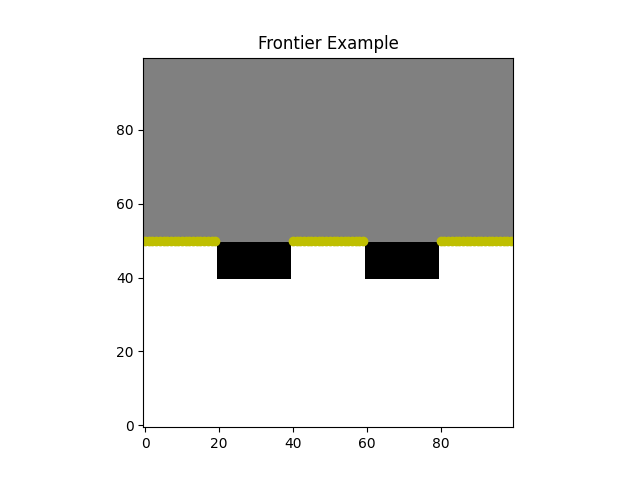
\includegraphics[width=8cm]{Images/frontier_example.png}
\end{center}

Clearly, there exist two distinct frontiers. By applying DBSCAN (Density-Based Spatial Clustering of Applications with Noise) to the frontier cells,
we can group them together, and identify centroids of each frontier.

\begin{center}
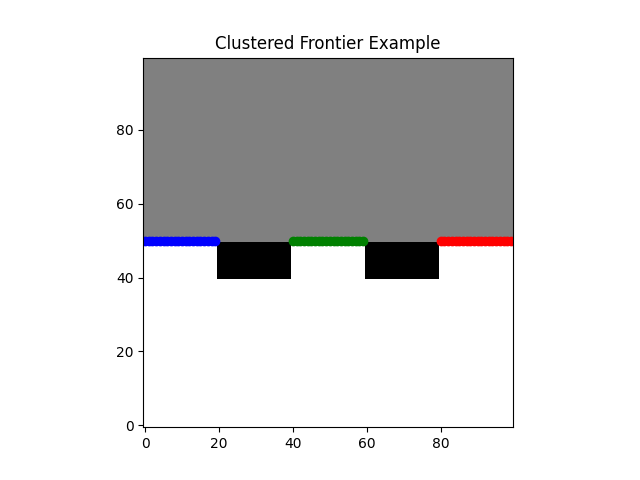
\includegraphics[width=8cm]{Images/clustered_frontier_example.png}
\end{center}

Using this approach, we can reformulate the optimization problem to assign explorer agents to frontiers. 

This was the problem I ended up working on in the end, as I simply did not have time
in the scope of this project to complete work on everything outlined up to this point.

I instead streamlined the problem to focus on finding some kind of approximation
to the optimization problem outlined above. I propose the following greedy algorithm:

\begin{algorithm}
\caption{Greedy Frontier Assignment}
\begin{enumerate}
    \item Perform frontier clustering using DBSCAN
    \item Using Djikstra's, compute the shortest path for each agent to each frontier centroid
    \item While there are unassigned agents:
    \begin{enumerate}
        \item Assign the agent closest to a frontier centroid to that frontier
        \item Check if that assignment violates connectivity constraints
        \item If it does, move this agent to the back of the queue
        \item If not, remove that frontier from the list of frontiers
    \end{enumerate}
\end{enumerate}
\end{algorithm}

% REFERENCES

\bibliographystyle{IEEEtran}
\bibliography{IEEEabrv, main.bib}

\end{document}
